\documentclass[twocolumn]{article}

\usepackage{amstext}
\usepackage{amsmath}
\usepackage{graphicx}
\usepackage{float}
\usepackage{caption}
\usepackage{subcaption}
\usepackage[margin=1in, paperwidth=8.5in, paperheight=11in]{geometry}
%\usepackage{gensymb}
\usepackage{here}
\usepackage{caption}

\usepackage[backend=biber]{biblatex}
\addbibresource{references.bib}

\def\changemargin#1#2{\list{}{\rightmargin#1\leftmargin#2}\item[]}
\let\endchangemargin=\endlist
\begin{document}

\title{Wolbachia and Two Other Microbes Nobody Cares About That Changed The World Kinda}
    \author{C. Bekins, R. Chapman and B. Wasti}
    \date{December 2015}
    \maketitle

\section*{Introduction}
\section*{Wolbachia}
\textit{Wolbachia} is a group of bacteria that infects arthropod species. Technically there is only one true type of \textit{Wolbachia}, \textit{Wolbachia pipientis}, but due to the genetic diversity of different strains, it is commonly split into two groups, group A and group B, although it is generally just referred to as \textit{Wolbachia}.

The bacteria is found in the ovaries and testes of a wide range of arthropods.\cite{Wbio} It is passed on via reproduction, and can only be spread through females. \textit{Wolbachia} are considered mutualistic endosymbionts, and are "required for survival of their hosts."\cite{Wdisc_nem} An interesting thing to note is how universal \textit{Wolbachia}seems to be. It has been demonstrated that\textit{Wolbachia} infects 25-70\% of species of insects.\cite{Wdisc_nem}

To give a bit of background,\textit{Wolbachia} was first discovered by Samuel Burt Wolbach and described by Marshall Hertig in 1924.\cite{Winit} Wolbach had been studying the cause of Rocky Mountain Spotted Fever and by 1916 had shown that \textit{Dermacentor andersoni}, a tick native to the Rocky Mountain area, was the transmitter of the disease.\cite{wolbachia} He was unable to grow the actual bacteria causing the disease, a species of\textit{Rickettsia}, in a cell-free culture leading "him to speculate as to the relationship between the cells of the host and the intracellular parasites."\cite{wolbachia} This is important to note, because the discovery of\textit{Wolbachia} is closely linked to this idea.

Hertig came to work with Wolbach, and together they investigated a bacteria living in the gonads of the\textit{C. pipiens} mosquito. This bacteria is known today as\textit{Wolbachia pipientis} which Hertig gave a detailed description of in 1936.\cite{Wdiscription} At this point scientists did not know of the gene manipulation that\textit{Wolbachia} has on it's hosts, and the discovery largely went unnoticed.

During the 1950s a group of scientists found that certain matching between\textit{Culex} mosquitos produced no offspring. They named this phenomenon cytoplasmic incompatibility, although they were not sure as to what the cause was.\cite{Wcyto_iso} It wasn't until the 1970s that cytoplasmic incompatibility was linked to\textit{Wolbachia}, when a group of scientists eliminated the\textit{Wolbachia} through antibiotics.\cite{Wcyto_cause}

Also during the 1960s and '70s scientists noted "unusual structures in the oocytes or in the hypodermis" of filarial nematodes but did not associate them with bacteria.\cite{wolbachia} It wasn't until 1995 that these "unusual structures" were determined to be\textit{Wolbachia}.\cite{Wstruct} 

The history of\textit{Wolbachia} is rather curious, and for good reason. On the surface,\textit{Wolbachia} are just harmless bacteria living in the reproductive areas of different insects that don't really do anything. But only recently has it been shown that\textit{Wolbachia} has shaped the world in drastic ways, and is one of the most prolific parasitic bacteria.\cite{Wdistr}

There is a very good reason for the abundance of\textit{Wolbachia}, for better or for worse, it completely hijacks the host organism's reproductive organs. One of the most unique features of\textit{Wolbachia} is the reproductive changes it makes in its host species. It can cause cytoplasmic incompatibility \cite{Wci0}\cite{Wci1}\cite{Wci2}\cite{Wci3}, parthenogenesis \cite{Wparth}, feminization of males \cite{Wfem} and male killing.\cite{Wmale_killing} All of these different changes force the host species to pass on\textit{Wolbachia} to their offspring, also known as vertical transfer.

%##### How does it function?
The most prominent of these reproductive changes is cytoplasmic incompatibility which is a "reproductive incompatibility between sperm and egg."\cite{Wbio} \textit{Wolbachia} can only be passed on through eggs, and not sperm, so in order to get around this limitation it has evolved to not allow inter-breeding between members of the same species where only one of them is infected with\textit{Wolbachia}. However, it gets even more complicated than this.

There are actually two types of cytoplasmic incompatibility, unidirectional and bidirectional. Unidirectional allows an infected female to mate with an uninfected male, which makes sense because the\textit{Wolbachia} can still be passed on. Bidirectional cytoplasmic incompatibility occurs when there is no case where an infected member and an uninfected member can mate succesfuly. The reason for these two different 'modes' is even more complicated still.

It goes back to the idea that there are two separate groups of\textit{Wolbachia}, group A and group B. Comparing the 16S rDNA does not give a full picture for the genetic diversity of the\textit{Wolbachia}, and the ftsZ gene was used to compare the genetics of 38 different\textit{Wolbachia} strains.\cite{Wgenetics} It was found that there is in fact a very large genetic difference between strains, and that group A and group B diverged 58-67 million years ago. 

\begin{figure}[!ht]
    \centering
    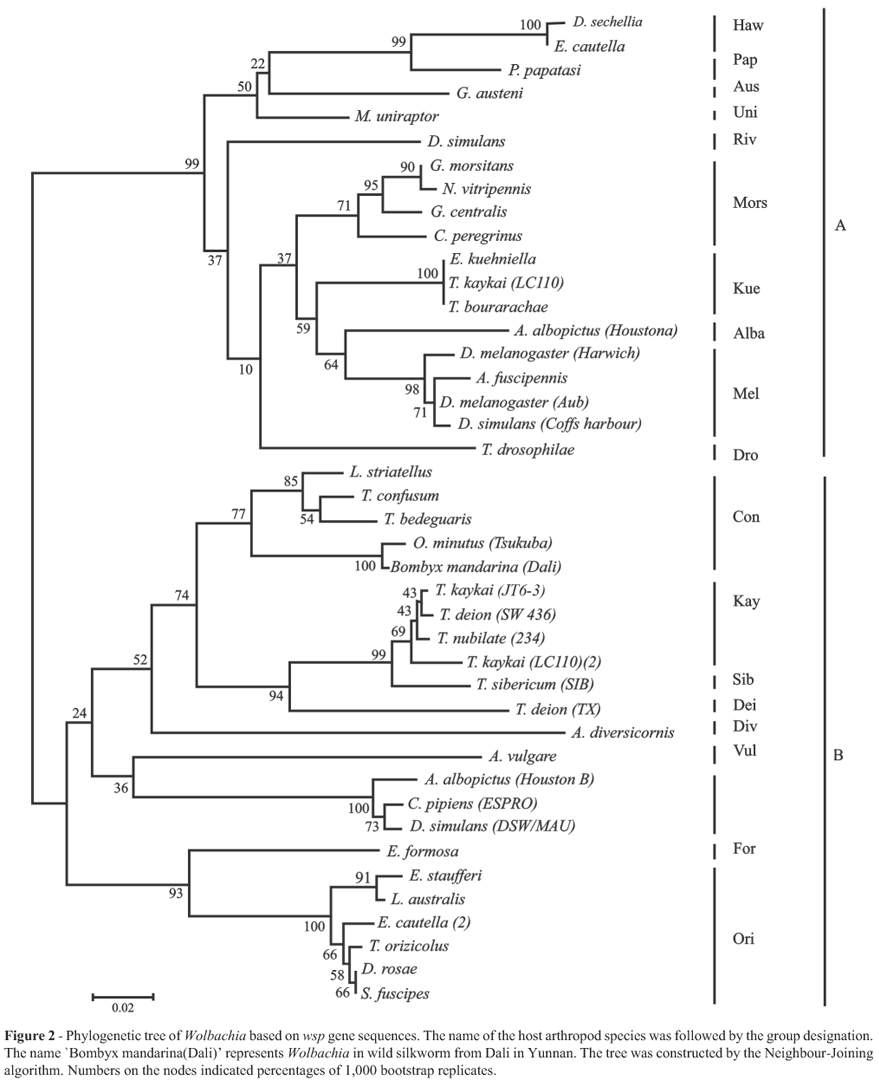
\includegraphics[width=.4\textwidth]{images/WolbachiaTree.jpg}
    \caption{ ... }
    \label{fig:wolbachiha_tree}
\end{figure}

Going back to cytoplasmic incompatibility, when a species is infected with two different strains of\textit{Wolbachia} (a species can in fact be infected with multiple strains) that are mutually incompatible, bidirectional cytoplasmic incompatibility occurs.\cite{WbiCI} It makes more sense when discussing how\textit{Wolbachia} cause this cytoplasmic incompatibility.

The exact mechanisms for the cause of cytoplasmic incompatibility are not known. What is known is that the\textit{Wolbachia} in the male modify the sperm in such a way that only if the same strain of\textit{Wolbachia} is in the female species to "recover" the sperm will correct fertilization occur.\cite{Wbio}

In many ways\textit{Wolbachia} acts like an encryption algorithm, "encrypting" the sperm sent to the female, and only if the female has the correct decryption algorithm can she get pregnant. This is also why different strains of\textit{Wolbachia} are incompatible, using a wrong decryption algorithm will generate nonsense.

The other unique reproductive change\textit{Wolbachia} causes is parthogenisis, or the ability for unfertilized eggs to grow into healthy adults essentially eliminating the need for males in a species. This makes sense,\textit{Wolbachia} can only be passed on through females, so it does not care about the males. But then one might realize that\textit{Wolbachia} took over the male's job, and took millions of years of evolution for sexual differentiation and threw it out the window.

Perhaps the most famous case of parthogenisis caused by\textit{Wolbachia} is in the\textit{Trichogramma} wasps, where all members of the species are female. Weirdly, by treating the wasps with antibiotics to kill of the\textit{Wolbachia} cause "some female parthenogenetic strains ... to revert to production of male progeny."\cite{Wpar_removal} It would appear that\textit{Wolbachia} is merely surpressing the need for male's in certain species. Even stranger is the fact that "phylogenetic evidence suggests that [parthogenisis] has evolved several times independently in these bacteria" which, as one scientist puts it, suggests "a simple biochemical mechanism."\cite{Wbio}  

Despite the fact that we still do not know the exact biochemical mechanism that causes parthogenisis, we do know that it is the result of gamete duplication.\cite{Wgamete_duplication} There is still work to be done in order to figure out how\textit{Wolbachia} is inducing gamete duplication.

\section*{Toxoplasma}

\section*{Cordyceps}
Cordyceps, or more specifically \textit{Ophiocordyceps unilateralis}, is a fungus that infects ants. Otherwise known as a specialized fungal parasite. This zombifying, mind-controlling microbe is able to modify the behavior of its host. Eventually it kills its host in a location optimal for its reproduction. 

The story of how \textit{Ophiocordyceps} functions is a cycle, so you could start talking about it anywhere, but from an ant's perspective everything starts when it comes into contact with the spores of the fungus. The spores recognize they are on a host, and form a biological drill that utilizes enzymes and mechanical pressure to breach the ant's tough exoskeleton. Once inside, the fungus transforms into a yeast-like state, living in the hemocoel of the ant.\cite{cordy_infection} This is where the highly specialized adaptations of \textit{Ophiocordyceps} start to shine. There are many things that are unknown about how \textit{Ophiocordyceps} manipulates the mind of its host, but the outcome has been studied in depth. \textit{Ophiocordyceps} leads its host ant to the northern side of a sapling approximately 25 cm above the ground. There, the ant closes it mandibles on the bark of the sapling or the main vein on the bottom side of a leaf, never to open them again. It is there that the fungus rapidly colonizes the host, restructuring all nutrients available inside the host to produce a large fruiting body which grows out of the back of the ants head that will produce the spores to restart the cycle.\cite{life_of_dead_ant}

\begin{figure}[!ht]
    \centering
    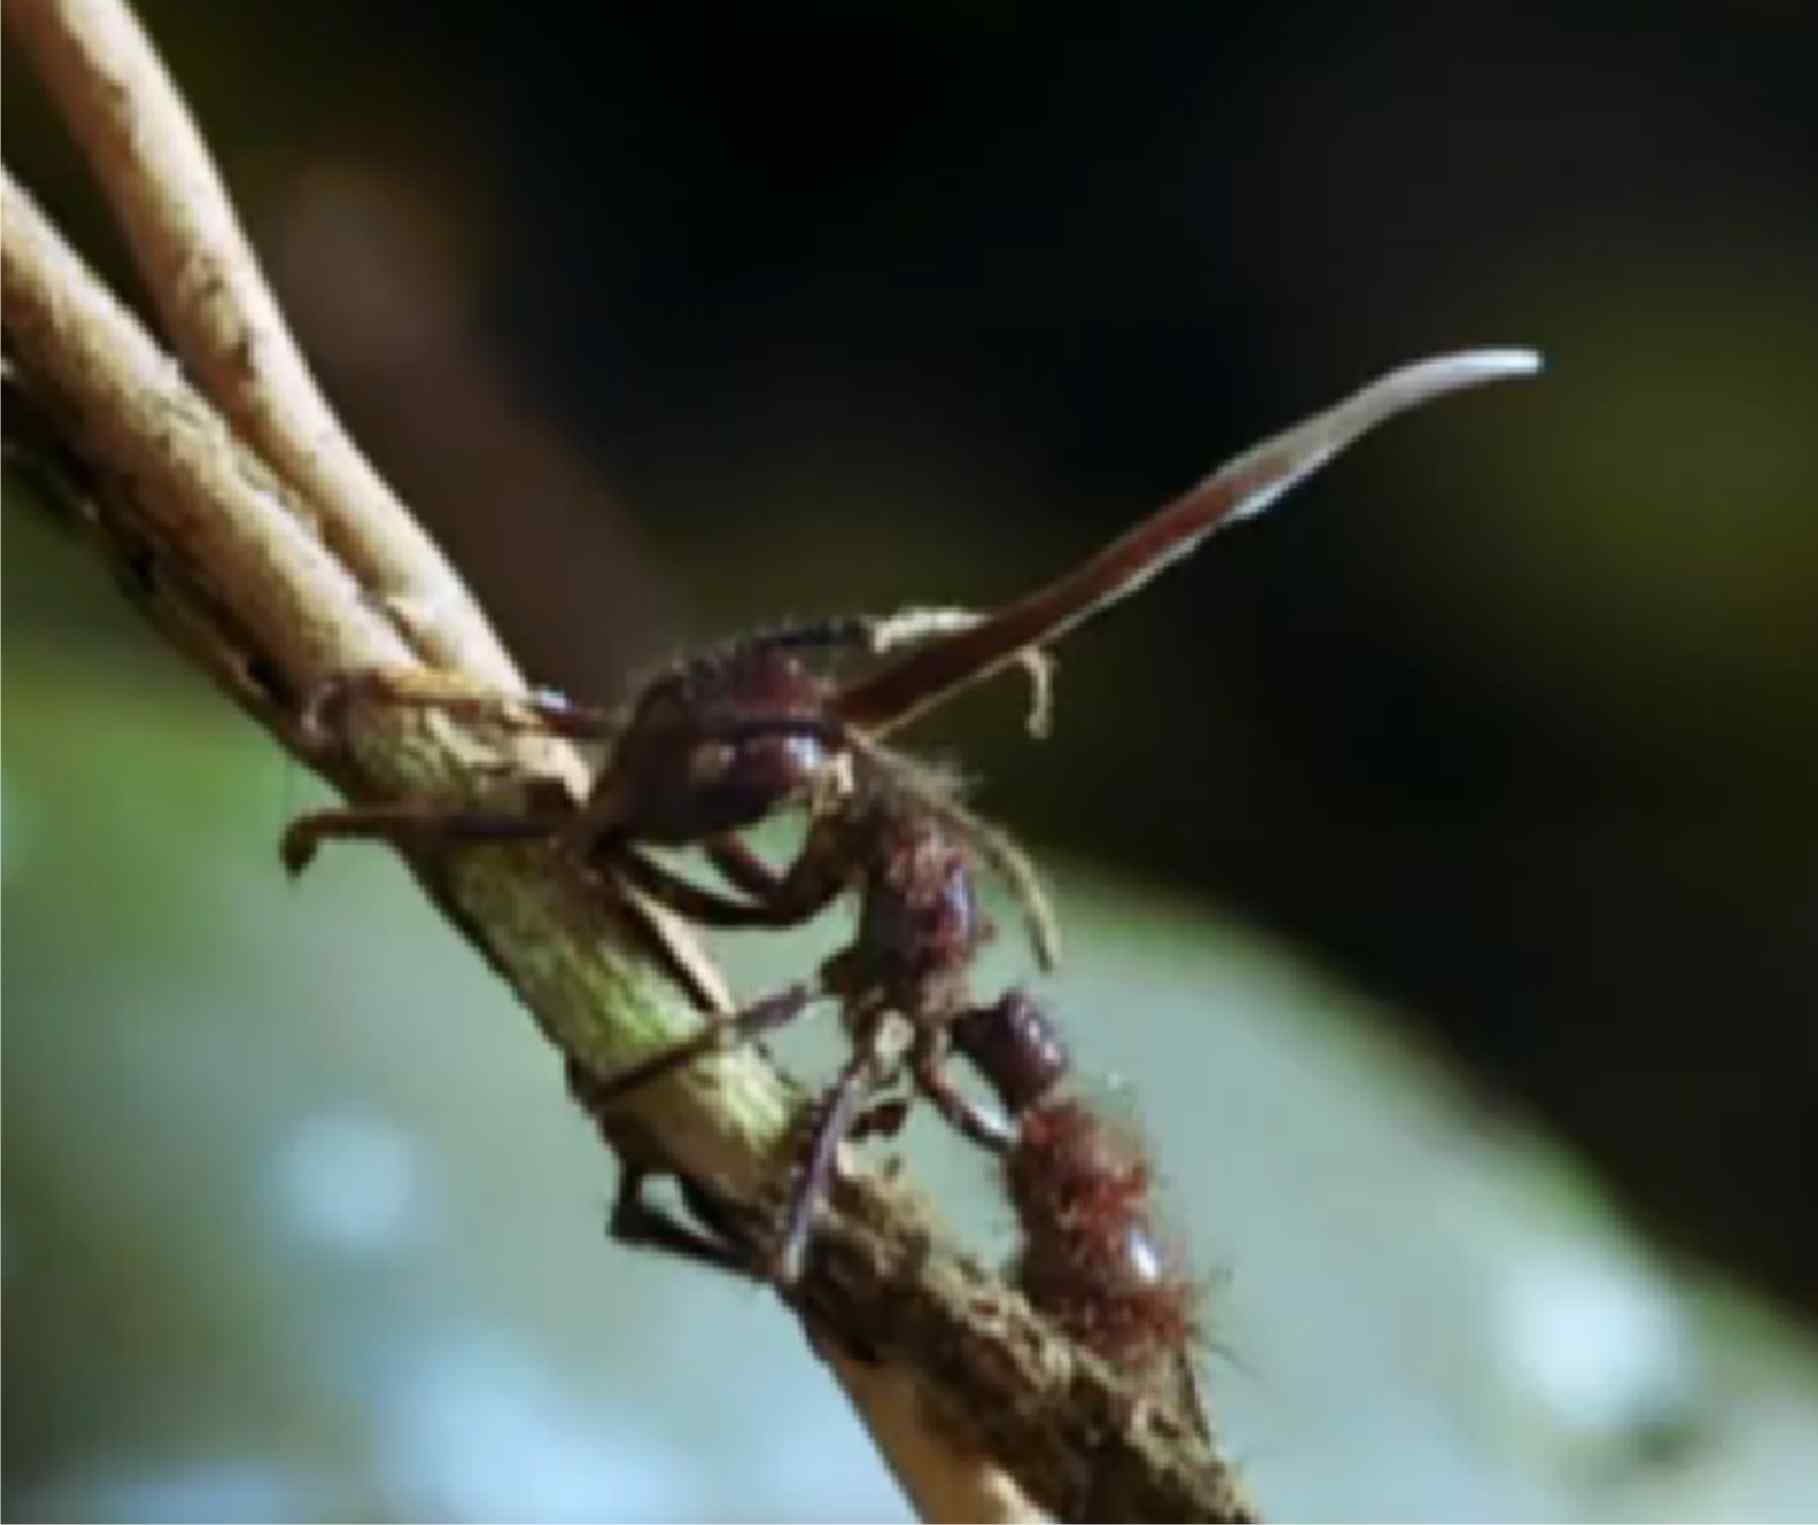
\includegraphics[width=.4\textwidth]{images/cordyceps_ant.jpg}
    \caption{The spore bearing fruiting body of \textit{Ophiocordyceps unilateralis} growing out of the back of the head of an ant whose mandibles are tightly gripping a twig. }
    \label{fig:cordyceps_ant}
\end{figure}

\section*{Impacts}

\section*{Analysis}

\section*{References}

\printbibliography

\end{document}
